\documentclass[11pt]{article}
\usepackage{adjustbox}
\usepackage{booktabs}
\usepackage{graphicx}
%\usepackage{subcaption}
\usepackage{caption}
\usepackage{mathtools}
\usepackage{tikz,pgfplots}
\usepackage{subfig}
\usepackage{epsfig}
\usepackage{amsmath}
\usepackage{amssymb}
\usepackage[shortlabels]{enumitem}
\usetikzlibrary{angles,patterns,calc}
\usepackage{bbm}
\usepackage{float}
\usepackage{natbib}
\usepackage[sc]{mathpazo}
\usepackage[T1]{fontenc}
\usepackage{amsfonts}
\usepackage[onehalfspacing]{setspace}
\usepackage[margin=.75in, tmargin=0.71in, bmargin=0.71in]{geometry}
\usepackage{url}
\usepackage{appendix}
\usepackage{hyperref}
\usepackage{xcolor}
\usepackage{todonotes}
\usepackage{lscape}
\usepackage{comment}
\newcommand\der[2]{\frac{\partial{#1}}{\partial{#2}}}
\DeclareMathOperator*{\argmax}{arg\,max}
\DeclareMathOperator*{\argmin}{arg\,min}

% stuff to put matlab code in 
\usepackage{listings}
\usepackage{color} %red, green, blue, yellow, cyan, magenta, black, white
\definecolor{mygreen}{RGB}{28,172,0} % color values Red, Green, Blue
\definecolor{mylilas}{RGB}{170,55,241}

% Shortcut greek
\def\a{\alpha}
\def\b{\beta}
\def\g{\gamma}
\def\D{\Delta}
\def\d{\delta}
\def\z{\zeta}
\def\k{\kappa}
\def\l{\lambda}
\def\n{\nu}
\def\r{\rho}
\def\s{\sigma}
\def\t{\tau}
\def\x{\xi}
\def\w{\omega}
\def\W{\Omega}

\usepackage[autostyle, english = american]{csquotes}
\MakeOuterQuote{"}

\usepackage[utf8]{inputenc}
\usepackage[english]{babel}
\usepackage{fancyhdr}
\fancypagestyle{firststyle}
{
\fancyhf{}
    \renewcommand{\headrulewidth}{0pt}
   \fancyfoot[C]{\footnotesize Page \thepage\ of \pageref{LastPage}}
}

\newcommand{\numpy}{{\tt numpy}}    % tt font for numpy

\topmargin -.5in
\textheight 9in
\oddsidemargin -.25in
\evensidemargin -.25in
\textwidth 7in

\newcommand{\question}[1]{ \begin{center} \noindent\colorbox{gray!10}{
\parbox{0.8\textwidth}{\vspace{0.125in} #1 \vspace{0.125in} } } \end{center} }

\begin{document}

    \thispagestyle{firststyle}

    \author{Isaac Liu, Nicol\'as Martorell \& Paul Opheim}
    \title{Principal Component Regression as a Solution to Measurement Error Bias} 
    \maketitle

    % code

    \lstset{language=Matlab,%
        %basicstyle=\color{red},
        breaklines=true,%
        morekeywords={matlab2tikz},
        keywordstyle=\color{blue},%
        morekeywords=[2]{1}, keywordstyle=[2]{\color{black}},
        identifierstyle=\color{black},%
        stringstyle=\color{mylilas},
        commentstyle=\color{mygreen},%
        showstringspaces=false,%without this there will be a symbol in the places where there is a space
        numbers=left,%
        numberstyle={\tiny \color{black}},% size of the numbers
        numbersep=9pt, % this defines how far the numbers are from the text
        emph=[1]{for,end,break},emphstyle=[1]\color{red}, %some words to emphasise
        %emph=[2]{word1,word2}, emphstyle=[2]{style},    
    }

    \begin{abstract}

        We argue that using Principal Component Regression (PCR) is a useful solution to bias introduced by measurement error in the covariate included in a regression. We show its usefulness through econometric theory and then use Monte Carlo simulations to show how it provides benefits for different parameters and correlations between the true covariate and the variable of interest. We then apply this method to study the relationship between life expectancy and the level of government involvement in a country's healthcare system.
        
    \end{abstract}

    \newpage \clearpage

    \section*{Introduction}

        Many variables of interest in economics are not directly available as empirical data. Instead, economists often use other variables that are imperfect measurements of the true focus of their analysis. These available variables are known as \textit{proxies} or ``variables measured with error'', and, if they suffer from classical measurement error, their use causes \textit{attenuation bias} when they are used as independent variables in econometric estimation. Traditionally, instrumental variables are used as a shock of exogeneity to get rid of this bias, but finding truly exogenous variables that satisfy the exclusion restriction is difficult, and so this method can often not be feasibly applied.

        As an alternative to dealing with attenuation bias, we propose the use of Principal Component Analysis (PCA) over several variables measured with error. When there are multiple observed variables driven by a single ``true'' one, we propose to use PCA over these variables to extract the ``true'' variable. We then use this extracted value and use it in a standard OLS regression, thus providing a solution to attenuation bias that does not require the strong assumptions of instrumental variable analysis.

        This estimator ties into earlier literature considering the intersection of factor models and principal components analysis and measurement error and latent variables problems. Somewhat similarly to our methods, \cite{nagasawa_identication_2020} develops the use of a proxy variable to deal with unobserved heterogeneity in nuisance parameters and uses a partial effects method. Differing from our setting, \cite{schennach_recent_2016} focuses on nonclassical measurement error and nonlinear cases and notes the usefulness of factor methods and some cases where they are of more use than instrumental variables. \cite{wegge_local_1996} considers a setting in which measurement error regression models are factor analysis models, with the correct regressors being the factors. Latent factors are uncorrelated with the errors. Focusing on measurement error in the main regressor, \cite{schofield_correcting_2015} combines solutions from structural equations modelling and item response theory to deal with misestimation. Finally, \cite{heckman_matching_2010} considers a situation similar to ours, except involving matching estimators. In this case, these estimators can be harmed by mismeasured conditioning variables. However, average treatment effects can be identified using factor proxies, and without need for normalization.

        In this paper, in order to show the properties and behaviour of our estimator on large samples under standard assumptions, we present a theoretical framework and a Monte-Carlo analysis. Additionally, we explore a basic empirical application to our method, by estimating the effect of economic development on life expectancy at birth. Since there is no consensus on how to measure economic development, we take a sample of different variables that may measure economic development with error (GDP per capita, GNI per capita, Household Income Per Capita, among others) over which we apply PCA to apply our identification strategy. Our estimator generally behaves as expected in this empirical setting, though it is unclear whether it performs any better or worse than other methods such as the direct inclusion of covariates or their averaging.

    \section*{Theoretical framework}

        Consider a model where the outcome is denoted by $y_i$. This outcome depends on a variable of interest denoted by $t_i$ and a vector of covariates denoted by $X_i=(x_{i,1},x_{i,2},\dots x_{i,p})'$. Additionally, consider a vector of variables $X^*_i=(x^*_{i,1},x^*_{i,2},\dots x^*_{i,p})'$ that correspond to the covariates $X_i$ but observed with measurement error, where $x^*_{i,k}=x_{i,k}+\eta_{i,k}$ with $\eta_{i,k} \sim {iid}(0,\sigma^2_{\eta_k})$, $\operatorname{E}(x_{i,k}'\eta_{i,k})=0, \forall i$, $\operatorname{E}(x_{i,k}'\eta_{j,l})=0, \forall i\neq j$ and $k \neq l$, and $\operatorname{E}(\eta_{i,k}'\eta_{j,l})=0, \forall i\neq j$ and $k \neq l$. Therefore, each $x^*_{i,k}$ suffers classical measurement error. Note that $\operatorname{E}(x_{i,k})=\operatorname{E}(x^*_{i,k})=\mu_{x_k}$ and that $\operatorname{V}(x_{i,k})=\sigma^2_{x_k}$ while $\operatorname{V}(x^*_{i,k})=\sigma^2_{x_k}+\sigma^2_{\eta_k}\geq \sigma^2_{x_k}$.

    \subsection*{Data Generation Process}

        Assume that the outcome $y_i$ is determined by the following Data Generation Process (DGP):
        \begin{align}
            y_i = \gamma t_i + X_i'\beta + \epsilon_i
        \end{align}

        where $\g$ is the parameter of the variable of interest $t_i$, $\b=(\b_1,\b_2,\dots \b_p)'$ is the vector of the parameters of the covariates $X_i$ including a constant and $\epsilon_i \sim \operatorname{iid}(0,\sigma^2_\epsilon)$. Under this specification, the coefficients are such that:
        \begin{align}
            \left(\begin{array}{l}
        {\gamma} \\
        {\beta}
        \end{array}\right)=\left(\begin{array}{cc}
        {\sigma}^2_{t} & \Sigma_{tX} \\
        \Sigma_{Xt} & {\Sigma}_{X}
        \end{array}\right)^{-1}\left(\begin{array}{c}
        \Sigma_{yt} \\
        \Sigma_{yX}
        \end{array}\right)
        \end{align}

        Suppose that the econometrician has access to $t_i$ but, instead of $X_i$ she observes $X^*_i$. Then, she specifies the following linear model
        \begin{align}
            y_i = \gamma^* t_i + {X^{*}_i}' \beta^* + \zeta_i
        \end{align}

        the coefficients would be such that
        \begin{align}
            \left(\begin{array}{l}
        {\gamma}^* \\
        {\beta}^*
        \end{array}\right)&=\left(\begin{array}{cc}
        {\sigma}^2_{t} & \Sigma_{tX^*} \\
        \Sigma_{X^*t} & {\Sigma}_{X^*}
        \end{array}\right)^{-1}\left(\begin{array}{c}
        \Sigma_{yt} \\
        \Sigma_{yX^*}
        \end{array}\right) \\
        & =\left(\begin{array}{cc}
        {\sigma}^2_{t} & \Sigma_{tX} \\
        \Sigma_{Xt} & {\Sigma}_{X}+{\Sigma}_{\eta}
        \end{array}\right)^{-1}\left(\begin{array}{cc}
        {\sigma}^2_{t} & \Sigma_{tX} \\
        \Sigma_{Xt} & {\Sigma}_{X}
        \end{array}\right)\left(\begin{array}{l}
        {\gamma} \\
        {\beta}
        \end{array}\right)
        \end{align}

        Without loss of generality, assume that the abovementioned DGP consists only of two variables as follows

            \begin{align}
                    y_i = \gamma^* t_i +  \beta^*x_i* + \zeta_i
                \end{align}

            Then, equations $(4)$ and $(5)$ will be such that
            \begin{align}
                    \left(\begin{array}{l}
                {\gamma}^* \\
                {\beta}^*
                \end{array}\right)&=\left(\begin{array}{cc}
                {\sigma}^2_{t} & \operatorname{cov}({t,x^*}) \\
                \operatorname{cov}({x^*,t}) & {\sigma}_{x^*}^2
                \end{array}\right)^{-1}\left(\begin{array}{c}
                \operatorname{cov}{(y,t)} \\
                \operatorname{cov}{(y,x^*)}
                \end{array}\right) \\
                \end{align}
            
            Thus, the coefficient of our variable of interest will be
            \begin{align}
            {\gamma}^* =\frac{\sigma_{x^*}^2\operatorname{cov}{(y,t)}-\operatorname{cov}({t,x^*})\operatorname{cov}{(y,x^*)}}{\sigma_{t}^2\sigma_{x^*}^2-\operatorname{cov}({t,x^*})^2}
        \end{align}

        And then
        \begin{align}
            \gamma^* = \gamma + \beta\frac{\operatorname{cov}(t,x)(\sigma^2_{x^*}-\sigma^2_x)}{\sigma_{t}^2\sigma_{x^*}^2-\operatorname{cov}({t,x})^2}
        \end{align}

        From $(10)$ it is clear that when $\operatorname{cov}(t,x)\neq 0$ and that $x$ is measured with error (i.e $\sigma_{x^*}^2>\sigma_x^2)$, the coefficient of our variable of interest is biased. If $t$ and $x$ are independent, then measurement error in $x^*$ does not cause any bias. If there is no measurement error in $x^*$, then $\sigma^2_{x^*}=\sigma^2_x$ and so we would not be facing any kind of bias, as one would expect.\\

        Equation $(10)$ also allows us to know the direction of the bias. Given that we are facing measurement error in the covariate, $\sigma^2_{x^*}>\sigma^2_x$ which implies $\sigma^2_{x^*}-\sigma^2_x>0$. Also, it follows from the \textit{Cauchy-Schwarz} inequality that the denominator is also positive. Then, the direction of the bias will depend on the sign of $\beta$ and the covariance of $t$ and $x$, as Table one illustrates.

        \begin{table}[h!]
            \centering
            \begin{tabular}{|c|c|c|}\hline \hline
            & $\b>0$  & $\b<0$ \\ \hline
            $\operatorname{cov}(t,x)>0$ & upward-biased & downward-biased \\ \hline
            $\operatorname{cov}(t,x)<0$ & downward-biased & upward-biased \\ \hline
            \end{tabular} 
            \caption{Direction of the Bias due to Measurement Error in the Covariate}
            \label{tab:my_label}
        \end{table}

        For a more concrete example, consider a simple case where the DGP depends only of the variable of interest and a covariate such that:

        \begin{align}
            \left(\begin{array}{l}
        {\gamma} \\
        {\beta}
        \end{array}\right)=\left(\begin{array}{l}
        1 \\
        1
        \end{array}\right)
        \end{align}

        and with $\sigma^2_t=\Sigma_X=\Sigma_\eta=1$ while $\Sigma_{Xt}=0.6$. Then
        \begin{align*}
            \left(\begin{array}{l}
        {\gamma}^* \\
        {\beta}^*
        \end{array}\right)& =\left(\begin{array}{cc}
        1 & 0.6 \\
        0.6 & 2
        \end{array}\right)^{-1}\left(\begin{array}{cc}
        1 & 0.6 \\
        0.6 & 1
        \end{array}\right)\left(\begin{array}{l}
        1\\
        1
        \end{array}\right) \\
        \left(\begin{array}{l}
        {\gamma}^* \\
        {\beta}^*
        \end{array}\right)&=\left(\begin{array}{l}
        1.37 \\
        0.39
        \end{array}\right)
        \end{align*}

        Clearly, both coefficients shows bias when the econometrician assumes a DGP with $X_i^*$: while there is attenuation bias on the coefficient of the covariate, the coefficient of the variable of interest is biased upward given that both variable have positive correlation.

    \subsection*{Principal Component Regression as bias-correction method}

        The classical solution for the measurement-error induced bias in econometrics has been the usage of instrumental variables. However, finding reliable source of exogeneity is difficult, as is arguing for a suitable exclusion condition. Therefore, the use of IV as a bias-correction method should be taken with care given that its feasibilty is hard.\\

        Alternatively, we propose an alternative bias-correction method when there are several mismeasured variables for each covariate, that is when we have more than one $x_{i,k}^*$ for every $x_{i,k}$. Given that in all the miss-measured variables the underlying value is the real value, one could think of extracting the underlying true $x_{i,k}$ through a linear combination of the different $x_{i,k}^*$. Then, we could treat all the $x_{i,k}^*$ as variables that share compononents as follows
        \begin{align}
        h_{j}=\underset{h^{\prime} h=1, h^{\prime} h_{1}=0, \ldots, h^{\prime} h_{j-1}=0}{\operatorname{argmax}} \operatorname{var}\left[h^{\prime} X^*_k\right]  
        \end{align}


        where $h_j$ is the eigenvector of $\Sigma$ associated with the $j^{t h}$ ordered eigenvalue $\lambda_{j}$ of $\Sigma_{X^*_k}$, and the principal components of $X^*_k$ are $U_{j}=h_{j}^{\prime} X^*_k$, where $h_{j}$ is the eigenvector of $\Sigma$ associated with the $j^{t h}$ ordered eigenvalue $\lambda_{j}$ of $\Sigma$.\\

        Under our assumptions, the vector of mismeasured values $X^*_k$ of $x_{i,k}$, share only one principal component which is precisely $x_{i,k}$. Then, we only have one principal component, $x_{i,k}$, and so the $x_{i,k}$ is such that
        \begin{align}
            x_{i,k}=h_{k}^{\prime} X^*_k
        \end{align}

        Finally, we could then retrieve the vector of true variables $X_i$
        \begin{align}
            X_i=HX^*_i
        \end{align}

        where $H$ is a matrix such that
        \begin{align*}
            H=\left(\begin{array}{ccccc}
        h_1 & 0 & 0 & \dots & 0 \\
        0 & h_2 & 0 & \dots & 0 \\
        \vdots & \ddots & h_3 & \ddots & \vdots \\
        0 & \dots & \dots & \dots \ddots & h_p
        \end{array}\right)
        \end{align*}

        and $h_k$ is the vector of eigenvalues for the variable $x_{i,k}$.

        Our new linear model then would be
        \begin{align}
            y_i = \gamma^{PCR} t_i + H{X^*_i}'\beta^{PCR} + \epsilon_i
        \end{align}

        where the coefficients are as follows
        \begin{align}
            \left(\begin{array}{l}
        {\gamma}^{PCR} \\
        {\beta}^{PCR}
        \end{array}\right)&=\left(\begin{array}{cc}
        {\sigma}^2_{t} & \Sigma_{t,HX^*} \\
        \Sigma_{HX^*,t} & {\Sigma}_{HX^*}
        \end{array}\right)^{-1}\left(\begin{array}{c}
        \Sigma_{yt} \\
        \Sigma_{y,HX^*}
        \end{array}\right)\\
        &=\left(\begin{array}{cc}
        {\sigma}^2_{t} & \Sigma_{t,HX^*} \\
        \Sigma_{HX^*,t} & {\Sigma}_{HX^*}
        \end{array}\right)^{-1}\left(\begin{array}{cc}
        {\sigma}^2_{t} & \Sigma_{tX} \\
        \Sigma_{Xt} & {\Sigma}_{X}
        \end{array}\right)\left(\begin{array}{l}
        {\gamma} \\
        {\beta}
        \end{array}\right)\\
        &=\left(\begin{array}{l}
        {\gamma} \\
        {\beta}
        \end{array}\right)
        \end{align}

        where the last equality comes from $(13)$.

        Note that according to equation $(17)$, the true variable $x_{i,k}$ is a linear combination of the mismeasured variables that the researcher may have, were the weights are such that equation $(16)$ is satisfied. This allows us to think about other linear combination that could be used as a bias-correction method. In particular, take the case in which $h_k='(\frac{1}{n},\frac{1}{n},\dots,\frac{1}{n})$, where $h_k$ is a row vector of dimension $(1\times J)$, and $J$ is the amount of mismeasured variables for $x_{i,k}$. Then, equation $(17)$ will be
        \begin{align}
            \Tilde{x_{i,k}}&=\left(\begin{array}{cccc}
        \frac{1}{n} & \frac{1}{n} & \dots &\frac{1}{n} 
        \end{array}\right)\left(\begin{array}{l}
        x^*_{i,1} \\
        x^*_{i,2} \\
        \vdots \\
        x^*_{i,J} 
        \end{array}\right)\\
        &=\frac{1}{n}\sum_{j=1}^J x^*_{i,j}
        \end{align}

        That is, the average of the mismeasured variables for $x_{i,k}$ is a feasible linear combination that may correct for the missmeasuremnet bias problem.

    \section*{Estimation of the Principal Component Regression}

        Recall that the mismeasured variables are such that $x^*_{i,k}=x_{i,k}+\eta_{i,k}$. Then for every $i$, $X_i^*$ can we get
        \begin{align}
            X_i^* = X_i +\mu
        \end{align}

        and so we could interpret the vector of mismeasured variables $X^*_i$ as a factor model, in which the common factor is the vector of true variables $X_i$. This way, we could rewrite the model as follows
        \begin{align}
            y_i &= \gamma t_i + X_i'\beta + \epsilon_i \\
            X_i^* &= X_i +\mu
        \end{align}

        which is a factor-augmented regression model in which the common ``factors'' between the mismeasured variables of $x_{i,k}$ is in fact $x_{i,k}$. We estimate the model following two-stages. First, we estimate $X_i$ by factor regression. Then, the first-stage is the principal-components estimation
        \begin{align}
            \hat{X_i}=\hat{D}^{-1}X_i^*
        \end{align}
        The second step is to regress $Y_i$ on the estimated $\hat X_i$. Then, the coefficients would be
        \begin{align}
            \left(\begin{array}{l}
        \hat{\gamma}^{F} \\
        \hat{\beta}^{F}
        \end{array}\right)&=\left(\begin{array}{cc}
        \hat{\sigma}^2_{t} & \hat\Sigma_{t,\hat X} \\
        \hat \Sigma_{\hat X,t} & \hat {\Sigma}_{\hat X}
        \end{array}\right)^{-1}\left(\begin{array}{c}
        \hat \Sigma_{yt} \\
        \hat \Sigma_{y,\hat X}
        \end{array}\right)
        \end{align}

        Using the \textit{Frisch-Waugh-Lowell} decomposition
        \begin{align}
            \hat{\g}^F & = ((M_{\hat{X}}t)'M_{\hat{X}}t)^{-1}(M_{\hat{X}}t)'M_{\hat{X}}y
        \end{align}

        Where $M_{\hat{X}}=I-\hat{X}(\hat{X}'\hat{X})^{-1}\hat{X}'$. Then
        \begin{align}
            \hat{\g}^F & = ((M_{\hat{X}}t)'M_{\hat{X}}t)^{-1}(M_{\hat{X}}t)'M_{\hat{X}}(t\gamma  + X\beta + \epsilon) \\
            &=\gamma +((M_{\hat{X}}t)'M_{\hat{X}}t)^{-1}(M_{\hat{X}}t)'M_{\hat{X}}X\beta+((M_{\hat{X}}t)'M_{\hat{X}}t)^{-1}(M_{\hat{X}}t)'M_{\hat{X}}\epsilon
        \end{align}

    \section*{Properties of the Estimator: Monte Carlo Simulations}

        We then complement our theoretical analysis by using Monte Carlo Simulation to analyze the effects of using Principal Components Regression as a method of bias correction. For these simulations, we assume that the true DGP for the data is:

        $$y_i = \beta_1 x_i + \beta_2 z_i + u_i$$

        ...where $x_i$ and $z_i$ are single variables drawn from $\mathcal{N}(\begin{bmatrix} 0\\ 0 \end{bmatrix}, \begin{bmatrix} 1 & \rho\\ \rho & 1\end{bmatrix})$, where $\rho$ is some covariance between our main variable of interest ($x_i$) and the covariate ($z_i$). The $u_i$ is drawn from a white noise distribution ($\mathcal{N}(0,1)$) that is uncorrelated with both $x_i$ and $z_i$. We then assume (as with the theoretical analysis) that $z_i$ is not directly observable and instead the researchers only have access to $p$ many measurements $z_{i,j}^*$ where $z_{i,j}^* = z_i + \eta_j$ where $\eta_j$ is drawn from a white noise distribution $\mathcal{N}(\mathbf{0},\Sigma)$ where $\mathbf{0}$ is a p-vector and $\Sigma$ is a diagonal p by p matrix with only 1s on the diagonal.
        
        In our simulations, we assume default values of $\rho = 0.5$, $\beta_1 = \beta_2 = 1$, and $p=5$. We then vary each factor while holding the others fixed, and perform 1,000 simulations of the DGP followed by an OLS regression on either the PCA value from the p measurements of the true $z_i$, or on a single one of the measurements of $z_i$. For each simulation, we generate 2,000 observations of $y_i,x_i$,etc. Table \ref{sim_p_2_noexp} shows the results for different values of $p$.

        \begin{table}[!htbp] \centering
  \caption{Average Coefficients for Values of $p$ (No Transformation of Measurements) \label{sim_p_2_noexp}}
  \scalebox{0.75}{
    \begin{tabular}{@{\extracolsep{5pt}}lccccc}
\\[-1.8ex]\hline
\hline \\[-1.8ex]
& \multicolumn{4}{c}{\textit{Number of p}} \
\cr \
\\[-1.8ex] & 5 & 20 & 50 &\\
\hline \\[-1.8ex]
& \multicolumn{4}{c}{\textit{Coefficient on Main Variable}} \\
 PCA & 1.104 & 1.030 & 1.014 &\\
  & (0.027) & (0.026) & (0.026) &\\
  Single Measurement & 1.284 & 1.285 & 1.287 &  \\
  & (0.029) & (0.029) & (0.028) &\\
& \multicolumn{4}{c}{\textit{Mean Absolute Percentage Error}} \\
  PCA & 10.4\% & 3.3\% & 2.3\% &  \\
  Single Measurement & 28.4\% & 28.5\% & 28.7\%  & \\
\hline \\[-1.8ex]
Simulations & 1,000 & 1,000 & 1,000 & \\
\hline
\hline \\[-1.8ex]
\end{tabular}}
\end{table}

        We can see that using PCA to extract the latent covariate driving the mismeasured covariates noticeably outperforms using a single mismeasured covariate across several values of $p$. Both the average coefficient on $\beta_1$ obtained when including the PCA output in the regression, and the mean absolute percentage error obtained on the 1,000 simulations are both much closer to the target values with the PCA-based regression than with the single measurement regression. Additionally, we can see that as $p$ increases the estimated $\beta_1^*$ coefficient in the PCA regression gets steadily closer to the true $\beta_1$ value of 1. This trend could well continue as $p \to \infty$, but we did not simulate values greater than $p = 50$ due to the seeming implausibility of having more than 50 measurements of the same single covariate. Appendix 1 contains charts that show that this increase in performance is also true for different values of $\beta_1$ and $\beta_2$.

        However, there are certain circumstances where the PCA method does not lead to more accurate estimates of $\beta_1^*$. Table \ref{sim_rho_2_noexp} contains the simulation results for different values of $\rho$ (the covariance between the main variable of interest $x_i$ and the true latent covariate $z_i$):

        \begin{table}[!htbp] \centering
  \caption{Average Coefficients for Values of $\rho$ (No Transformation of Measurements) \label{sim_rho_2_noexp}}
\begin{tabular}{@{\extracolsep{5pt}}lccccc}
\\[-1.8ex]\hline
\hline \\[-1.8ex]
& \multicolumn{5}{c}{$\rho$ \textit{ Value}} \
\cr \
\\[-1.8ex] & -0.9 & -0.5 & 0 & 0.5 & 0.9 \\
\hline \\[-1.8ex]
& \multicolumn{5}{c}{\textit{Coefficient on Main Variable}} \\
 PCA & 0.538 & 0.894 & 1.000 & 1.104 & 1.464  \\
  & (0.039) & (0.027) & (0.024) & (0.027) & (0.041)\\
  Single Measurement & 0.244 & 0.714 & 1.000 & 1.284 & 1.759  \\
  & (0.030) & (0.029) & (0.027) & (0.028) & (0.031)\\
& \multicolumn{5}{c}{\textit{Absolute Percentage Error}} \\
  PCA & 46.2\% & 10.6\% & 1.9\% & 10.4\% & 46.4\% \\
   & (3.9 ppts) & (2.7 ppts) & (1.4 ppts) & (2.7 ppts) & (4.1 ppts)\\
  Single Measurement & 75.6\% & 28.6\% & 2.2\% & 28.4\% & 75.9\%  \\
  & (3.0 ppts) & (2.9 ppts) & (1.6 ppts) & (2.8 ppts) & (3.1 ppts)\\
\hline \\[-1.8ex]
 Observations & 1,000 & 1,000 & 1,000 & 1,000 & 1,000\\
\hline
\hline \\[-1.8ex]
\end{tabular}
\end{table}


        We first note that when $\rho = 0.5$ then the coefficient on the variable of interest is artificially inflated when we use a single mismeasurement as a covariate (on average, 1.28 instead of the true value of 1). Conversely, when $\rho = -0.5$ then the coefficient is artificially deflated. Using the PCA value as the covariate reduces this bias for both directions, and brings the main coefficient closer to its true value of 1.0. These results are consistent with our theoretical section, where we argued that a positive covariance between the main variable and the true covariate will lead to an inflation on the main coefficient, while a negative covariance will lead to a deflation of the coefficient. Separately, there is very little bias when $\rho = 0$, as predicted in the theory section. Since there is hardly any bias to correct, we do not see gains from using the PCA covariate method for that particular $\rho$ value. Also, when $\rho = -1$ or $1$, there is no notable improvement from using the PCA-extracted latent variable (and notice that since the variances of $x_i$ and $z_i$ are 1, this means that the covariance is equal to the correlation in these simulations). These simulation results suggest that so long as the correlation between $x_i$ and $z_i$ is not close to $-1$, $0$, or $1$, there are noticeable performance gains from using PCA to extract the true covariate from a collection of observed variables that try to measure that true covariate.
        
        However, the performance advantages that we see from using PCA could be driven by the benefit of having multiple measurements of our true covariate of interest, as opposed to any special advantages from PCA specifically. We test this question by comparing the estimated $\beta_1^*$ in our PCA regressions with the estimated $\beta_1^*$ when we include all $p$ measurements as separate covariates in the regression, and the $\beta_1^*$ obtained when the covariate is the mean of all $p$ measurements of the true covariate. The results from these regressions for different values of $p$ are shown in Table \ref{sim_p_4_noexp}.

        \begin{table}[!htbp] \centering
  \caption{Average Coefficients for Values of p (No Transformation of Measurements) \label{sim_p_4_noexp}}
\begin{tabular}{@{\extracolsep{5pt}}lccccc}
\\[-1.8ex]\hline
\hline \\[-1.8ex]
& \multicolumn{4}{c}{\textit{Number of p}} \
\cr \
\\[-1.8ex] & 5 & 20 & 50 \\
\hline \\[-1.8ex]
& \multicolumn{4}{c}{\textit{Coefficient on Main Variable}} \\
PCA & 1.104 & 1.030 & 1.014 &\\
& (0.027) & (0.026) & (0.026) &\\
All Measurements & 1.104 & 1.030 & 1.013  \\
  & (0.027) & (0.022) & (0.018)\\
 Average of Measurements & 1.104 & 1.030 & 1.013  \\
  & (0.027) & (0.022) & (0.017)\\
  Instrumental Variable & 1.125 & 1.037 & 1.029 \\
& (0.028) & (0.026) & (0.026) \\
& \multicolumn{4}{c}{\textit{Absolute Percentage Error}} \\
PCA & 10.4\% & 3.3\% & 2.3\% &  \\
& (2.7 ppts) & (2.2 ppts) & (1.8 ppts) &\\
All Measurements & 10.4\% & 3.3\% & 2.3\%  \\
  & (2.7 ppts) & (2.2 ppts) & (1.8 ppts)\\
  Average of Measurements & 10.4\% & 3.3\% & 2.3\%  \\
  & (2.7 ppts) & (2.2 ppts) & (1.7 ppts)\\
  Instrumental Variable & 12.5\% & 3.9\% & 3.2\% \\
& (2.8 ppts) & (2.4 ppts) & (2.2 ppts) \\
\hline \\[-1.8ex]
 Observations & 1,000 & 1,000 & 1,000  \\
\hline
\hline \\[-1.8ex]
\end{tabular}
\end{table}

        As one can see from these results (and results for different values of $\beta_1$, $\beta_2$, and $\rho$ in Appendix 2), there does not seem to be a noticeable difference between these three regression methods (across any values of $p, \beta_1,\beta_2$, and $\rho$. Thus, our simulations suggest that there are major benefits to having multiple measurements of a latent covariate of interest, but that using PCA, taking the average of these measurements, and including all measurements as separate covariates seem to give similar benefits to the performance of the regression.

        \begin{table}[!htbp] \centering
  \caption{Average Coefficients for Values of $p$ (Half of Measurements are Transformed) \label{sim_p_5_exp}}
  \scalebox{0.75}{
    \begin{tabular}{@{\extracolsep{5pt}}lccccc}
\\[-1.8ex]\hline
\hline \\[-1.8ex]
& \multicolumn{4}{c}{\textit{Number of p}} \
\cr \
\\[-1.8ex] & 5 & 20 & 50 \\
\hline \\[-1.8ex]
& \multicolumn{4}{c}{\textit{Coefficient on Main Variable}} \\
PCA & 1.208 & 1.082 & 1.054\\
& (0.032) & (0.029) & (0.028)\\
Single Measurement & 1.286 & 1.286 & 1.286 &  \\
& (0.029) & (0.029) & (0.028) &\\
All Measurements & 1.182 & 1.057 & 1.024  \\
  & (0.029) & (0.027) & (0.026)\\
 Average of Measurements & 1.365 & 1.303 & 1.285  \\
  & (0.034) & (0.029) & (0.028)\\
  Instrumental Variable & 1.234 & 1.065 & 1.039 \\
  & (0.029) & (0.027) & (0.026) \\
  
& \multicolumn{4}{c}{\textit{Absolute Percentage Error}} \\
PCA & 20.8\% & 8.2\% & 5.5\%  \\
& (3.2 ppts) & (2.9 ppts) & (2.7 ppts)\\
Single Measurement & 28.6\% & 28.6\% & 28.6\%  & \\
& (2.9 ppts) & (2.9 ppts) & (2.8 ppts) &\\
All Measurements & 18.2\% & 5.8\% & 2.9\%  \\
  & (2.9 ppts) & (2.6 ppts) & (2.1 ppts)\\
  Average of Measurements & 36.5\% & 30.3\% & 28.5\%  \\
  & (3.4 ppts) & (3.3 ppts) & (3.2 ppts)\\
  Instrumental Variable & 23.4\% & 6.5\% & 4.1\% \\
  & (2.9 ppts) & (2.7 ppts) & (2.4 ppts) \\
  
\hline \\[-1.8ex]
 Observations & 1,000 & 1,000 & 1,000  \\
\hline
\hline \\[-1.8ex]
\end{tabular}}
\end{table}

    \section*{Application: Government Share of Healthcare Spending and Life Expectancy}

        We now examine the implications of the principal components estimator in an empirical setting with measurement error. One interesting question in public economics and public health is the study of the effect of publicly and privately funded healthcare systems on outcomes such as life expectancy. To measure the public or private nature of a healthcare system we use the continuous variable of the government's share of total health expenditure in a given country and year.

        Some previous work has covered this relationship. Considering that this topic has been studied in "relatively few papers," \cite{linden_life_2017} focus on the relationship between life expectancy at birth and public and private health expenditures for 34 OECD countries from 1970-2012 and find that both public and private health spending are important to life expectancy and are associatied with each other. Other studies find a variety of effects; considering developing nations in Africa, \cite{novignon_effects_2012} finds a larger impact for public spending while \cite{filmer_impact_1999} finds no impact; in the developed US and Canada, \cite{lichtenberg_sources_2005} finds an impact only for public spending on outcomes when controlling for lagged GDP, while \cite{cremieux_public_2005} finds private spending on drugs is more effective. In the most similar work to ours, \cite{or_determinants_2000} predicts premature death in 21 OECD countries from 1970-1992, considering the public share of health expenditure, environmental factors, and GDP. He finds that a larger share of public spending is associated with lower rates of premature mortality for both males and females, and that controlling for GDP is important; it is also associated with less premature mortality. This work also demonstrates the importance of our methods of reducing the number of covariates considered, as it includes many economic variables and fixed effects but examines only several hundred observations; the estimators used may be subject to an important amount of variance.

        In this regression it is important to account for the role of a country's level of economic development. There is an extensive literature documenting the relationship between economic development and life expectancy. \cite{ling_testing_2017} finds that economic growth is associated with increased life expectancy in Malaysia, while considering the reversed causal direction \cite{acemoglu_disease_2007} finds improvements in life expectancy lead to little or no growth. Somewhat less obvious is the linkage between government provision of healthcare and development. In general, public goods provision and government spending, including in fields such as healthcare, has been linked to prosperity; low income countries may remain in such a state due to inefficient governments and inferior institutions \citep{wu_impact_2010}.

        However, economic development is liable to be measured with error. GDP measurements usually rely on company surveys, and the methodology within a country and for comparisons between countries through exchange rates or PPP adjustments may vary \citep{grishin_main_2019}. Other sources of error include the presence of the informal economy and non-monetary but productive work, the challenge of accurately measuring the value of digital services which often do not have visible prices, and government incentives to manipulate official statistics about growth \citep{charmes_informal_2012,ahmad_can_2017,nakamura_are_2016}.\footnote{Due to differences in statistical capacity and the larger relative size of the informal economy, it is possible that mismeasurement of economic development is particularly severe in developing countries. On the other hand, the presence of the digital economy may mean mismeasurement is larger in developed nations. This would constitute the presence of non-classical measurement error, but we only consider classical measurement error in this paper.} Hence, this setup, with a covariate in regression subject to measurement error, fits the situation described in the theory and simulations in the previous sections.\footnote{It seems less likely that our variable of interest, the government's share of health spending, is measured with error. One would think most governments capable of monitoring their own spending better than economic activity in general. Furthermore, for this variable there would seem to be less governmental incentive to manipulate the statistic.} In this case, we aim to to reduce possible bias in the coefficient of the government's share of health spending by making appropriate use of multiple measures of economic development.

        Our data on all measures comes from the World Bank, though we also make usage of OECD government health share data to fill in missing years, and average World Bank and OECD measurements when both are available \citep{the_world_bank_indicators_2021,oecd_oecd_2021}. We standardize all variables by subtracting the mean and dividing by the standard deviation, linearly interpolate data between known observations, and remove country-years with missing values for any of the economic indicators.

        In Table \ref{main_regs} below we begin with a univariate OLS regression, which produces a large and significant coeffcient indicating a one standard deviation increase in the government share of health expenditure is linked to a 0.268 standard deviation increase in life expectancy. Next we include the potentially mismeasured covariate of GDP per capita, which greatly reduces the size of the coefficient on the governments share. After this we include a full set of economic covariates listed in the upper rows of Table \ref{Sum_Stats}, again reducing the size of the coefficient. However, this result is then adjusted upwards again in the last two columns, where use the mean of the mismeasured covariates, and the first principal component.

        \begin{table}[!htbp] \centering
  \caption{Regressions of Life Expectancy on Government Share of Health Spending \label{main_regs}}
\begin{tabular}{@{\extracolsep{5pt}}lccccc}
\\[-1.8ex]\hline
\hline \\[-1.8ex]
& \multicolumn{5}{c}{\textit{Life Expectancy at Birth (Years)}} \
\cr \
\\[-1.8ex] & (1) & (2) & (3) & (4) & (5) \\
\hline \\[-1.8ex]
 Govt. Share of Health Exp. & 0.671$^{***}$ & 0.485$^{***}$ & 0.409$^{***}$ & 0.443$^{***}$ & 0.443$^{***}$ \\
  & (0.013) & (0.014) & (0.015) & (0.015) & (0.015) \\
 Covariates & None & GDP PC PPP & Econ Indicators & Mean & PC 1 \\
\hline \\[-1.8ex]
 Observations & 3,427 & 3,427 & 3,427 & 3,427 & 3,427 \\
 $R^2$ & 0.450 & 0.523 & 0.547 & 0.538 & 0.538 \\
 Adjusted $R^2$ & 0.450 & 0.522 & 0.547 & 0.538 & 0.538 \\
 Residual Std. Error & 0.742 & 0.691 & 0.674 & 0.680 & 0.680  \\
 F Statistic & 2800.594$^{***}$  & 1873.795$^{***}$  & 689.111$^{***}$  & 1997.019$^{***}$  & 1996.565$^{***}$  \\
\hline
\hline \\[-1.8ex]
\textit{Note:} & \multicolumn{5}{r}{$^{*}$p$<$0.1; $^{**}$p$<$0.05; $^{***}$p$<$0.01} \\
\end{tabular}
\end{table}
        
        \begin{table}
\centering
\caption{Summary Statistics}
\label{Sum_Stats}
\begin{tabular}{lcccccc}
\toprule
                                    Variable &  Obs &     Mean &       SD &     Min &      Med &       Max \\
\midrule
GDP Per Capita PPP (Current International \$) & 3427 & 17148.93 & 18949.29 & 435.08 & 10476.79 & 141634.96 \\
GDP Per Capita (Current USD) & 3427 & 12799.04 & 17699.30 & 111.93 & 4513.61 & 118823.65 \\
GNP Per Capita PPP (Current International \$) & 3427 & 16678.40 & 18229.65 & 410.00 & 10170.00 & 132440.00 \\
GNP Per Capita (Current USD) & 3427 & 12312.02 & 16773.90 & 110.00 & 4320.00 & 104560.00 \\
ILO GDP Per Person Employed & 3427 & 45084.61 & 40659.73 & 1371.24 & 32843.69 & 266953.37 \\
Life Expectancy at Birth (All Population) & 3427 & 70.15 & 9.14 & 39.44 & 72.50 & 84.36 \\
Government Share of Health Expenditure & 3427 & 51.86 & 22.15 & 4.06 & 53.38 & 95.14 \\
\bottomrule
\end{tabular}
\end{table}


        The results clearly demonstrate that all of the methods using multiple measures of the covariates produce noticably different coefficients for government health share. The usage of many economic indicators directly, the mean, and the principal components estimator each produce smaller coefficients.

        Moreover, these different coefficients behave in a manner similar to that predicted by our theoretical development and simulations. In Table \ref{sim_rho_2_noexp}, we saw the impact of variation in $\rho$, the correlation between measurements for a value of $p = 5$ and $\beta = 1$ for 100 observations. In the empirical setting it is difficult to tell what is a reasonable value of $\beta$, and we instead have nearly 2000 observations. Nevertheless, we see that for a positive $\rho$ value between 0 and 1 (as is likely to be the case in light the correlation between GDP and the government share of health spending and overall public goods), the coefficient obtained from using a single measurement is inflated relative to that from PCA, and presumably other methods combining multiple measures as in columns (3), (4), and (5) of Table \ref{main_regs}.

        Results using fixed effects panel models (with country clustered standard errors), more principal components, and instrumental variables regression of using all the economic indicators as an instrument for GDP per capita, are in Table \ref{additional_regs}. Fixed effects coefficients greatly reduce the magnitude of effects. Including more principal components and the instrumental variables technique produce coefficients of moderate size close to that obtained by the single principal component. The results in column (3) and (4) also show reductions in the inflation of coefficients relative to column (2) of Table \ref{main_regs}.

        \begin{table}[!htbp] \centering
  \caption{Additional Regressions \label{additional_regs}}
\begin{tabular}{@{\extracolsep{5pt}}lcccc}
\\[-1.8ex]\hline
\hline \\[-1.8ex]
& \multicolumn{4}{c}{\textit{Life Expectancy at Birth (Years)}} \
\cr \
\\[-1.8ex] & (1) & (2) & (3) & (4) \\
\hline \\[-1.8ex]
 Govt. Share of Health Exp. & -0.003$^{}$ & -0.008$^{}$ & 0.444$^{***}$ & 0.483$^{***}$ \\
  & (0.026) & (0.026) & (0.015) & (0.014) \\
 Covariates & None & PC 1 & PC 1-2 & GDP PC (IV) \\
 Fixed Effects & Yes & Yes & No & No \\
\hline \\[-1.8ex]
 Observations & 3,427 & 3,427 & 3,427 & 3,427 \\
 $R^2$ & 0.980 & 0.980 & 0.539 & 0.523 \\
 Adjusted $R^2$ & 0.979 & 0.978 & 0.538 & 0.522 \\
 Residual Std. Error & 0.145 & 0.147 & 0.680 & 0.691  \\
 F Statistic & 9487.991$^{***}$  & 19554.057$^{***}$  & 1331.968$^{***}$  & nan$^{***}$  \\
\hline
\hline \\[-1.8ex]
\textit{Note:} & \multicolumn{4}{r}{$^{*}$p$<$0.1; $^{**}$p$<$0.05; $^{***}$p$<$0.01} \\
\end{tabular}
\end{table}

    \section*{Conclusion}
        
        Discuss possible extensions

    \clearpage \newpage

    \bibliographystyle{aea}
    \bibliography{PCR_ME_Refs}

    \clearpage \newpage

    \appendix

    \section*{Appendix 1}

        \begin{table}[!htbp] \centering
  \caption{Average Coefficients for Values of $\beta_1$ (No Transformation of Measurements) \label{sim_beta1_5_noexp}}
  \scalebox{0.75}{
    \begin{tabular}{@{\extracolsep{5pt}}lccccc}
\\[-1.8ex]\hline
\hline \\[-1.8ex]
& \multicolumn{4}{c}{\textit{True $\beta_1$}} \
\cr \
\\[-1.8ex] & 0.1 & 1 & 10\\
\hline \\[-1.8ex]
& \multicolumn{4}{c}{\textit{Coefficient on Main Variable}} \\
 PCA & 0.205 & 1.104 & 10.106  \\
  & (0.026) & (0.027) & (0.027)\\
  Single Measurement & 0.384 & 1.284 & 10.286  \\
& (0.028) & (0.028) & (0.029)\\
 All Measurements & 0.205 & 1.104 & 10.106  \\
  & (0.026) & (0.027) & (0.027)\\
 Average of Measurements & 0.205 & 1.104 & 10.106  \\
  & (0.026) & (0.027) & (0.027)\\\
  Instrumental Variable & 0.225 & 1.125 & 10.126 \\
& (0.027) & (0.028) & (0.028) \\
& \multicolumn{4}{c}{\textit{Absolute Percentage Error}} \\
  PCA & 104.9\% & 10.4\% & 1.1\%  \\
   & (26.1 ppts) & (2.7 ppts) & (0.3 ppts)\\
   Single Measurement & 284.4\% & 28.4\% & 2.9\%  \\
& (28.2 ppts) & (2.8 ppts) & (0.3 ppts) \\
All Measurements & 104.7\% & 10.4\% & 1.1\%  \\
  & (26.1 ppts) & (2.7 ppts) & (0.3 ppts)\\
  Average of Measurements & 104.7\% & 10.4\% & 1.1\%  \\
  & (26.1 ppts) & (2.7 ppts) & (0.3 ppts)\\
  Instrumental Variable & 125.4\% & 12.5\% & 1.3\%  \\
& (26.6 ppts) & (2.8 ppts) & (0.3 ppts)\\

\hline \\[-1.8ex]
 Observations & 1,000 & 1,000 & 1,000 &\\
\hline
\hline \\[-1.8ex]
\end{tabular}}
\end{table}
        \begin{table}[!htbp] \centering
  \caption{Average Coefficients for Values of $\beta_2$ (No Transformation of Measurements) \label{sim_beta2_5_noexp}}
  \scalebox{0.75}{
    \begin{tabular}{@{\extracolsep{5pt}}lccccc}
\\[-1.8ex]\hline
\hline \\[-1.8ex]
& \multicolumn{4}{c}{\textit{True $\beta_1$}} \
\cr \
\\[-1.8ex] & 0.1 & 1 & 10\\
\hline \\[-1.8ex]
& \multicolumn{4}{c}{\textit{Coefficient on Main Variable}} \\
 PCA & 1.011 & 1.104 & 2.057  \\
  & (0.025) & (0.027) & (0.106)\\
  Single Measurement & 1.029 & 1.284 & 3.863  \\
& (0.024) & (0.028) & (0.159)\\
 All Measurements & 1.011 & 1.104 & 2.054  \\
  & (0.025) & (0.027) & (0.106)\\
 Average of Measurements & 1.011 & 1.104 & 2.054  \\
  & (0.025) & (0.027) & (0.106)\\\
  Instrumental Variable & 1.013 & 1.125 & 2.259 \\
& (0.025) & (0.028) & (0.116) \\
& \multicolumn{4}{c}{\textit{Absolute Percentage Error}} \\
  PCA & 2.2\% & 10.4\% & 105.7\%  \\
   & (1.6 ppts) & (2.7 ppts) & (10.6 ppts)\\
   Single Measurement & 3.2\% & 28.4\% & 286.3\%  \\
& (2.0 ppts) & (2.8 ppts) & (15.9 ppts) \\
All Measurements & 2.2\% & 10.4\% & 105.4\%  \\
  & (1.6 ppts) & (2.7 ppts) & (10.6 ppts)\\
  Average of Measurements & 2.2\% & 10.4\% & 105.4\%  \\
  & (1.6 ppts) & (2.7 ppts) & (10.6 ppts)\\
  Instrumental Variable & 2.3\% & 12.5\% & 125.9\%  \\
& (1.6 ppts) & (2.8 ppts) & (11.6 ppts)\\

\hline \\[-1.8ex]
 Observations & 1,000 & 1,000 & 1,000 & 1,000 &\\
\hline
\hline \\[-1.8ex]
\end{tabular}}
\end{table}
        \begin{table}[!htbp] \centering
  \caption{Average Coefficients for Values of $\rho$ (No Transformation of Measurements) \label{sim_rho_5_noexp}}
  \scalebox{0.75}{
    \begin{tabular}{@{\extracolsep{5pt}}lccccc}
\\[-1.8ex]\hline
\hline \\[-1.8ex]
& \multicolumn{5}{c}{$\rho$ \textit{ Value}} \
\cr \
\\[-1.8ex] & -1 & -0.5 & 0 & 0.5 & 1 \\
\hline \\[-1.8ex]
& \multicolumn{5}{c}{\textit{Coefficient on Main Variable}} \\
PCA & 0.538 & 0.894 & 1.000 & 1.104 & 1.464  \\
& (0.039) & (0.027) & (0.024) & (0.027) & (0.041)\\
Single Measurement & 0.244 & 0.714 & 1.000 & 1.284 & 1.759  \\
& (0.030) & (0.029) & (0.027) & (0.028) & (0.031)\\
All Measurements & 0.539 & 0.894 & 1.000 & 1.104 & 1.463  \\
  & (0.039) & (0.027) & (0.014) & (0.027) & (0.041)\\
 Average of Measurements & 0.539 & 0.894 & 1.000 & 1.104 & 1.463  \\
  & (0.039) & (0.027) & (0.014) & (0.027) & (0.041)\\
  Instrumental Variable & 0.487 & 0.874 & 1.000 & 1.125 & 1.514 \\
  & (0.038) & (0.027) & (0.024) & (0.028) & (0.040) \\

  & \multicolumn{5}{c}{\textit{Absolute Percentage Error}} \\
  PCA & 46.2\% & 10.6\% & 1.9\% & 10.4\% & 46.4\% \\
   & (3.9 ppts) & (2.7 ppts) & (1.4 ppts) & (2.7 ppts) & (4.1 ppts)\\
   Single Measurement & 75.6\% & 28.6\% & 2.2\% & 28.4\% & 75.9\%  \\
   & (3.0 ppts) & (2.9 ppts) & (1.6 ppts) & (2.8 ppts) & (3.1 ppts)\\
 All Measurements & 46.1\% & 10.6\% & 1.9\% & 10.4\% & 46.3\%  \\
  & (3.9 ppts) & (2.7 ppts) & (1.4 ppts) & (2.7 ppts) & (4.1 ppts)\\
  Average of Measurements & 46.1\% & 10.6\% & 1.9\% & 10.4\% & 46.3\% \\
  & (3.9 ppts) & (2.7 ppts) & (1.4 ppts) & (2.7 ppts) & (4.1 ppts)\\
  \hline \\[-1.8ex]
  Instrumental Variable & 51.3\% & 12.6\% & 2.0\% & 12.5\% & 51.4\% \\
  & (3.8 ppts) & (2.7 ppts) & (1.4 ppts) & (2.8 ppts) & (4.0 ppts) \\
  
 Observations & 1,000 & 1,000 & 1,000 & 1,000 & 1,000\\
\hline
\hline \\[-1.8ex]
\end{tabular}}
\end{table}
        
    \section*{Appendix 2}


         \begin{table}[!htbp] \centering
  \caption{Average Coefficients for Values of $\beta_1$ (Half of Measurements are Transformed)\label{sim_beta1_5_exp}}
  \scalebox{0.75}{
  \begin{tabular}{@{\extracolsep{5pt}}lccccc}
\\[-1.8ex]\hline
\hline \\[-1.8ex]
& \multicolumn{4}{c}{\textit{True $\beta_1$}} \
\cr \
\\[-1.8ex] & 0.1 & 1 & 10\\
\hline \\[-1.8ex]
& \multicolumn{4}{c}{\textit{Coefficient on Main Variable}} \\
 PCA & 0.307 & 1.208 & 10.205  \\
  & (0.032) & (0.032) & (0.032)\\
  Single Measurement & 0.385 & 1.286 & 10.284  \\
& (0.029) & (0.029) & (0.028)\\
 All Measurements & 0.281 & 1.181 & 10.180  \\
  & (0.028) & (0.029) & (0.027)\\
 Average of Measurements & 0.465 & 1.365 & 10.363  \\
  & (0.034) & (0.034) & (0.033)\\\
  Instrumental Variable & 0.333 & 1.234 & 10.232 \\
& (0.029) & (0.029) & (0.028) \\
& \multicolumn{3}{c}{\textit{Absolute Percentage Error}} \\
  PCA & 207.3\% & 20.8\% & 2.1\%  \\
   & (32.1 ppts) & (3.2 ppts) & (0.3 ppts)\\
   Single Measurement & 285.0\% & 28.6\% & 2.8\%  \\
& (28.6 ppts) & (2.9 ppts) & (0.3 ppts) \\
All Measurements & 181.3\% & 18.2\% & 1.8\%  \\
  & (27.9 ppts) & (2.9 ppts) & (0.3 ppts)\\
  Average of Measurements & 364.6\% & 36.5\% & 3.6\%  \\
  & (34.2 ppts) & (3.4 ppts) & (0.3 ppts)\\
  Instrumental Variable & 233.3\% & 23.4\% & 2.3\%  \\
& (28.8 ppts) & (2.9 ppts) & (0.3 ppts)\\

\hline \\[-1.8ex]
 Observations & 1,000 & 1,000 & 1,000 &\\
\hline
\hline \\[-1.8ex]
\end{tabular}}
\end{table}
        \begin{table}[!htbp] \centering
  \caption{Average Coefficients for Values of $\beta_2$ (Half of Measurements are Transformed) \label{sim_beta2_5_exp}}
  \scalebox{0.75}{
    \begin{tabular}{@{\extracolsep{5pt}}lccccc}
\\[-1.8ex]\hline
\hline \\[-1.8ex]
& \multicolumn{4}{c}{\textit{True $\beta_1$}} \
\cr \
\\[-1.8ex] & 0.1 & 1 & 10\\
\hline \\[-1.8ex]
& \multicolumn{4}{c}{\textit{Coefficient on Main Variable}} \\
 PCA & 1.021 & 1.208 & 3.091  \\
  & (0.025) & (0.032) & (0.214)\\
  Single Measurement & 1.029 & 1.286 & 3.871  \\
& (0.024) & (0.029) & (0.158)\\
 All Measurements & 1.018 & 1.182 & 2.826  \\
  & (0.025) & (0.029) & (0.129)\\
 Average of Measurements & 1.036 & 1.365 & 4.669  \\
  & (0.024) & (0.034) & (0.247)\\\
  Instrumental Variable & 1.023 & 1.234 & 3.347 \\
& (0.024) & (0.029) & (0.160) \\
& \multicolumn{4}{c}{\textit{Absolute Percentage Error}} \\
  PCA & 2.7\% & 20.8\% & 209.1\%  \\
   & (1.8 ppts) & (3.2 ppts) & (21.4 ppts)\\
   Single Measurement & 3.2\% & 28.6\% & 287.1\%  \\
& (2.0 ppts) & (2.9 ppts) & (15.8 ppts) \\
All Measurements & 2.5\% & 18.2\% & 182.6\%  \\
  & (1.8 ppts) & (2.9 ppts) & (12.9 ppts)\\
  Average of Measurements & 3.8\% & 36.5\% & 366.9\%  \\
  & (2.1 ppts) & (3.4 ppts) & (24.7 ppts)\\
  Instrumental Variable & 2.8\% & 23.4\% & 234.7\%  \\
& (1.9 ppts) & (2.9 ppts) & (16.0 ppts)\\

\hline \\[-1.8ex]
 Observations & 1,000 & 1,000 & 1,000 & 1,000 &\\
\hline
\hline \\[-1.8ex]
\end{tabular}}
\end{table}
        \begin{table}[!htbp] \centering
  \caption{Average Coefficients for Values of $\rho$ (Half of Measurements are Transformed) \label{sim_rho_5_exp}}
  \scalebox{0.75}{
    \begin{tabular}{@{\extracolsep{5pt}}lccccc}
\\[-1.8ex]\hline
\hline \\[-1.8ex]
& \multicolumn{5}{c}{$\rho$ \textit{ Value}} \
\cr \
\\[-1.8ex] & -1 & -0.5 & 0 & 0.5 & 1 \\
\hline \\[-1.8ex]
& \multicolumn{5}{c}{\textit{Coefficient on Main Variable}} \\
PCA & 0.337 & 0.793 & 0.997 & 1.208 & 1.663  \\
& (0.041) & (0.033) & (0.026) & (0.032) & (0.041)\\
Single Measurement & 0.244 & 0.716 & 0.997 & 1.286 & 1.757  \\
& (0.031) & (0.029) & (0.028) & (0.029) & (0.031)\\
All Measurements & 0.377 & 0.819 & 0.997 & 1.182 & 1.624  \\
  & (0.037) & (0.028) & (0.026) & (0.029) & (0.036)\\
 Average of Measurements & 0.177 & 0.637 & 0.998 & 1.365 & 1.822  \\
  & (0.030) & (0.034) & (0.029) & (0.034) & (0.030)\\
  Instrumental Variable & 0.302 & 0.768 & 0.998 & 1.234 & 1.698 \\
  & (0.035) & (0.030) & (0.027) & (0.029) & (0.035) \\
  
& \multicolumn{5}{c}{\textit{Absolute Percentage Error}} \\
  PCA & 66.3\% & 20.7\% & 2.1\% & 20.8\% & 66.3\% \\
   & (4.1 ppts) & (3.3 ppts) & (1.6 ppts) & (3.2 ppts) & (4.1 ppts)\\
   Single Measurement & 75.6\% & 28.4\% & 2.3\% & 28.6\% & 75.7\%  \\
   & (3.1 ppts) & (2.9 ppts) & (1.7 ppts) & (2.9 ppts) & (3.1 ppts)\\
 All Measurements & 62.3\% & 18.1\% & 2.1\% & 18.2\% & 62.4\%  \\
  & (3.6 ppts) & (2.8 ppts) & (1.6 ppts) & (2.9 ppts) & (3.6 ppts)\\
  Average of Measurements & 82.2\% & 36.3\% & 2.3\% & 36.5\% & 82.2\% \\
  & (3.0 ppts) & (3.4 ppts) & (1.8 ppts) & (3.4 ppts) & (3.0 ppts)\\
  \hline \\[-1.8ex]
  Instrumental Variable & 69.8\% & 23.2\% & 2.1\% & 23.4\% & 69.8\% \\
  & (3.5 ppts) & (3.0 ppts) & (1.6 ppts) & (2.9 ppts) & (3.5 ppts) \\
  
  Simulations & 1,000 & 1,000 & 1,000 & 1,000 & 1,000\\
\hline
\hline \\[-1.8ex]
\end{tabular}}
\end{table}


    \section*{Appendix 3}

        \begin{figure}[h!]
            \centering
            \caption{Correlations Between Covariates and Life Expectancy}
            \label{LE_Health_Econ_Correlations}	
            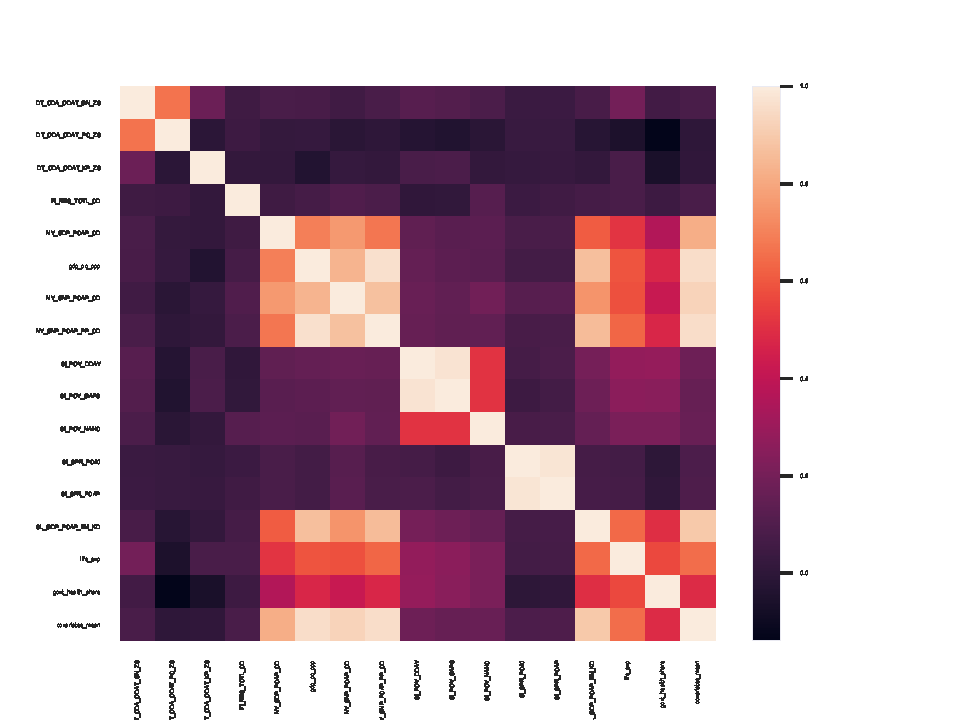
\includegraphics[width=\linewidth,keepaspectratio=true]{../Output/Figures/LE_Health_Econ_Correlations_combined_short.pdf}
        \end{figure}

        \begin{figure}[h!]
            \centering
            \caption{Economic Measures PCA Loadings}
            \label{Econ_Loadings}	
            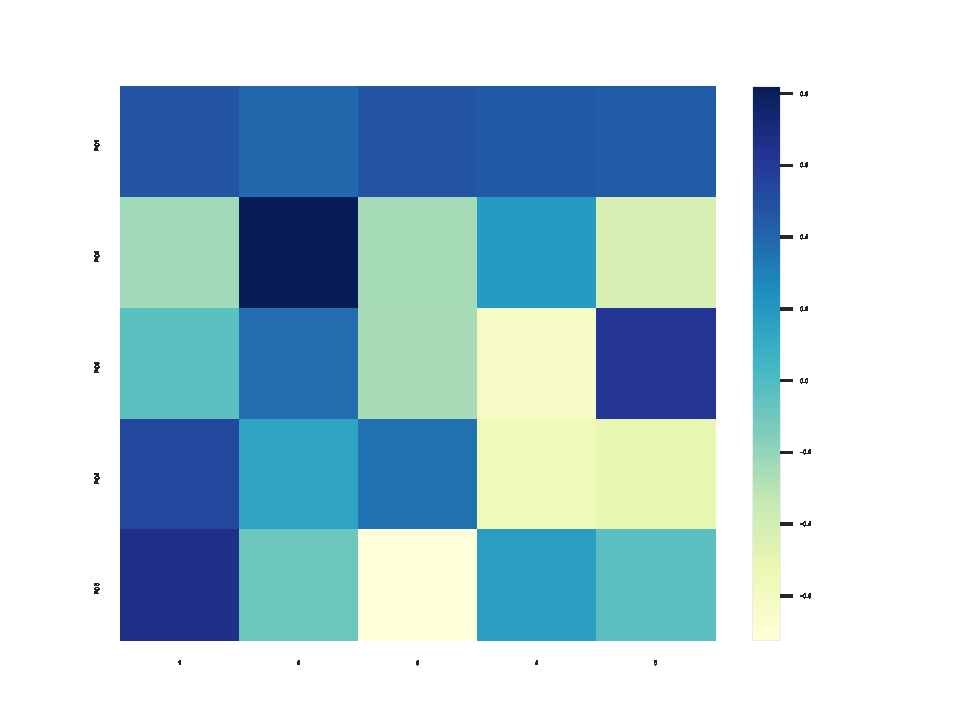
\includegraphics[width=\linewidth,keepaspectratio=true]{../Output/Figures/Econ_Indicator_Loadings_combined_short.pdf}
        \end{figure}

        \begin{figure}[h!]
            \centering
            \caption{Economic Measures PCA Share of Variance Explained}
            \label{Econ_Share_Explained}	
            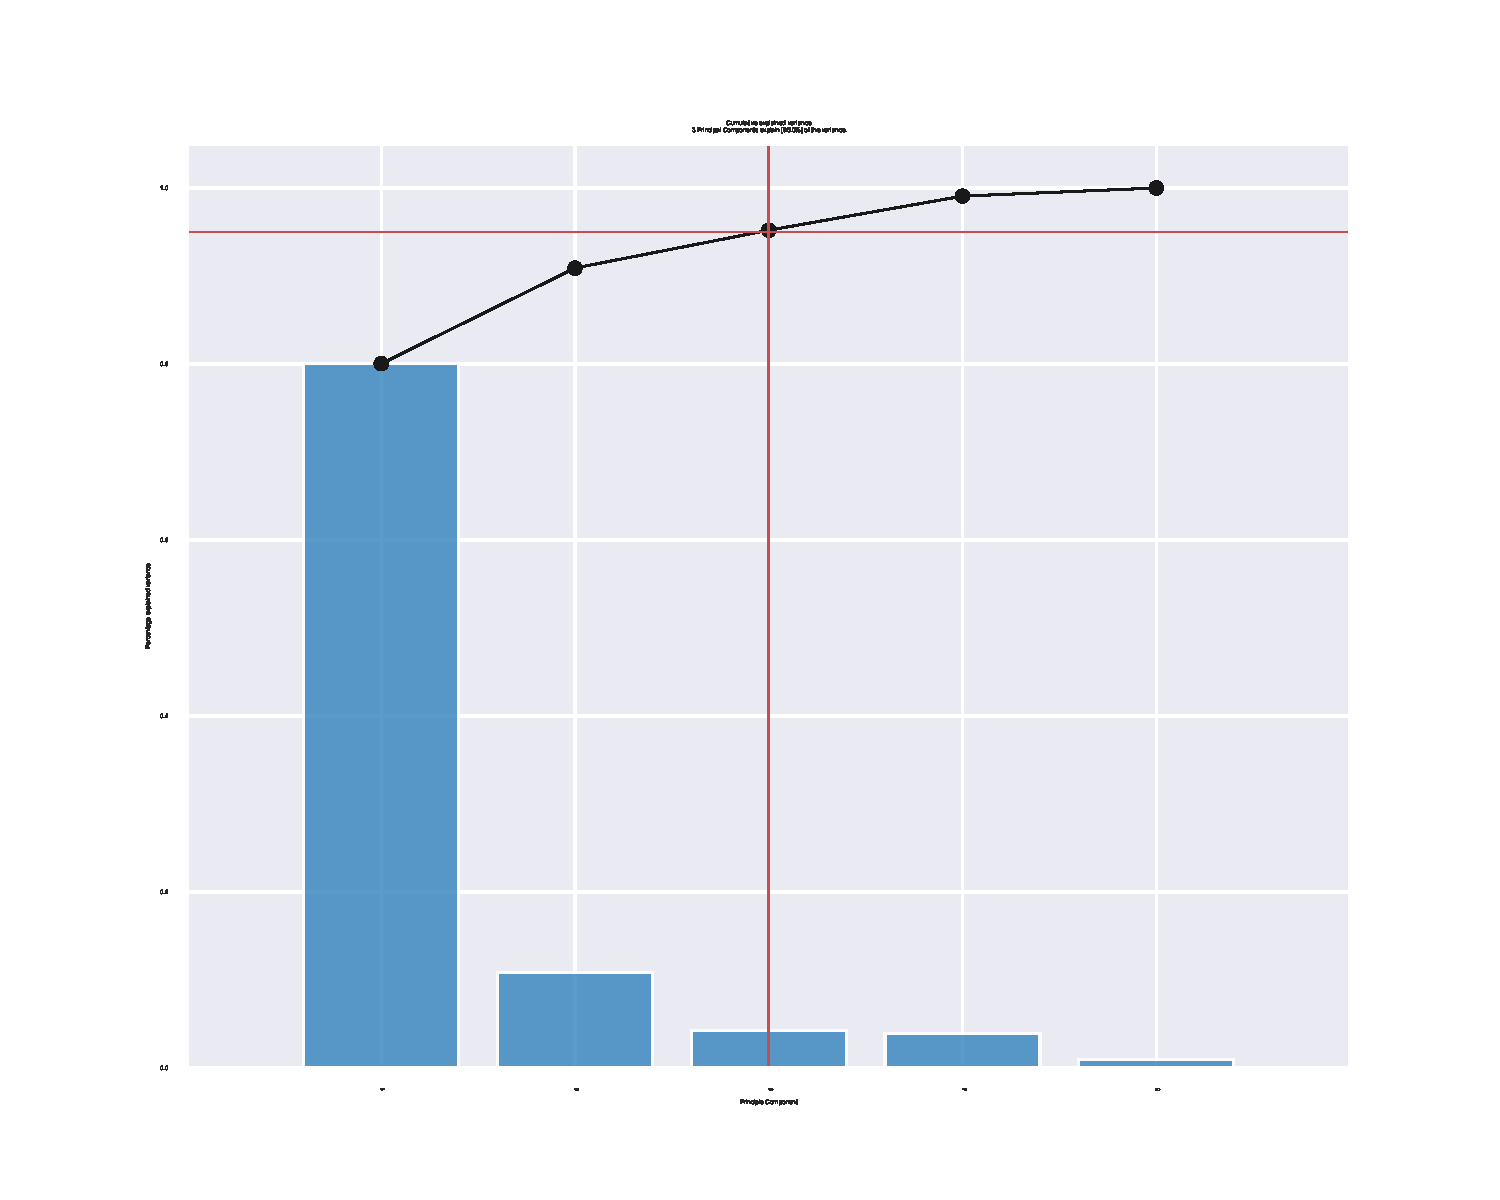
\includegraphics[width=\linewidth,keepaspectratio=true]{../Output/Figures/Econ_Indicator_Share_Explained_combined_short.pdf}
        \end{figure}

\end{document}